\documentclass{mcmthesis}
\bibliographystyle{plain}
\mcmsetup{CTeX = false,   % 使用 CTeX 套装时,设置为 true
        tcn = H155, problem = B,
        sheet = true, titleinsheet = true, keywordsinsheet = true,
        titlepage = false, abstract = true}
\usepackage{palatino}
\usepackage{lipsum}
\usepackage[UTF8, nocap]{ctex}
\usepackage{array}
\usepackage{float}
%\usepackage{ctex}
%\usepackage{CJK}
\title{The New Thermostat: Born to Know You Better}
\author{}
\date{\today}

\begin{document}

	\begin{abstract}
		
		Several conflicting criteria exist in smart house system design optimization, especially energy consumption and indoor environment thermal performance. This paper presents a novel model based on multi-objective optimization that can assist occupants in improving comfort, as well as energy conservation.
		
		We begin with the establishment of a mathematical model of one thermostat for single occupant. We decompose the whole controlling process into two parts: warming up preparation process and maintenance process. Both processes depend on four factors: architectural building design, system, environmental real-time data and occupants. Each process is an independent optimization model. 
		
		During the heating process, after learning the “you”, model adds environmental factors to dynamically adjusted itself iteratively. In the maintenance process, the ASHRAE-55 standard is used to obtain a set of optimal solutions after considering the person's preferences, and finally adding energy constraints to assist the thermostat's work. Both processes can be more energy efficient in the case of maintaining indoor thermal comfort conditions. For the above process, we did a lot of simulation experiments and compared it with other strategies.
		
		Next, we consider the situation where multiple people are in the same room at the same time. Under the consideration of fairness and game, the model eliminates the influence of personal preference on the model, and then uses the minimum enthalpy difference to select the minimum energy consumption strategy to achieve a comfortable environment. We verify the simulation from two indicators of energy saving effect and comfort performance.
		
		Thirdly, we know that it is not enough to use only one thermostat in a large house, so we introduce a multi-thermostat linkage model. We based on above model to calculate the most comfortable environment of each room, and then build a algorithm to consider the influence between rooms, using the total minimum energy consumption to achieve the comfortable balance of each room.
		
		Finally, effects of some special external factors are considered in our models. And we analyze the stability and sensitively of our models. Although there are some weakness in our models, the results still demonstrate that our model is considered and robust in certain extent.
		
		\begin{keywords}
			multi-objective optimization; least enthalpy; air conditioning; energy saving
		\end{keywords}
	\end{abstract}

	\maketitle
	\setcounter{tocdepth}{2}
	\tableofcontents
	
	
	\section{Introduction}
		
		Broadly speaking, a cozy living climate has become a necessity for almost every family. Modeling issues on better home climate control systems is, at root, modeling on comfort and electricity consumption optimization. In this problem, we need to consider a smart home climate control system under some specific situation. 
		
		\subsection{Problem Summary}
		
			To fulfill this, we decompose the problem into several steps:
			
			\begin{itemize}
				\item Build up a climate control system using a thermostat to meet needs and take energy consumption into consideration. Use it as framework for further analysis.
				\item Design a model dealing with diverse needs and preference from more than one individual. Estimate group comfort and costs.
				\item comprehensive comparison is made with two other smart home climate control systems currently in use.
				\item Establishing a combined working system of multiple thermostats.
				\item Implement sensitivity test and analyze model strengths and weaknesses.
			\end{itemize}
		
			
		\subsection{Our Starting Point: Existing Models}
		
			Studies of house climate control have been performed both operationally and theoretically by giant and innovative enterprise in the decades since its creation. These existing systems have been refined over time by our increasing needs for comfort, improved measuring tools, and the capabilities of modern computers.
			
			Before developing our own model, we explored the literature and on-line information to gain a thorough understanding of existing systems, and which complexities they consider. A few are highlighted here:
			
			
			\begin{itemize}
				\item Thermostats make a big step forward in intelligence and understanding of humans. Examples include:
				\item[-]Control your thermostat away from home using your phone.
				\item[-]Set a schedule for your heat.
				\item[-]Geofencing and motion detection, so it knows when you’re home (Note: The Ecobee4 uses IFTTT for geofencing) and can turn on the display when you walk by.
				\item[-]Smarter adjustment of switching time with historical information (learned from you).
				\item The existence of thermostats has made great progress in visualization and ease of operation due to market competition, but these are not the parts we want to explore and enhance, and there is not much discussion here.
			\end{itemize}
		
			We will present a more detailed analysis of the existing three thermostats below and a comprehensive comparison with our model.
		
		
		\subsection{Our Model}
		
			Our modeling approach is rooted in our conclusion that while these trend focuses on learning from history information of human, a full model of considering theoretical and live-data is necessary. People's habits, for instance, will prevent people from constantly changing to achieve the best environment because of laziness.
			
			Thus, our model will focus on implementing complexity where detail is most necessary, and simplicity where detail is not necessary, as determined by our research. 
			
			\textbf{We hope to obtain a smart climate control system through the preference of human, as well as accurate live-data and valid theory, but reduce the cost of electricity at the same time.} 
	
	\section{Fundamental Assumptions}
		\begin{itemize}
			\item When there is no one in the house, we assume that the house will soon return to the ambient climatic conditions.
			
			\item We consider air conditioning to adjust the temperature of indoor air, regardless of the heat absorbed by the indoor regenerator and the heat released by the indoor heat releaser.
			
			\item We assume that there is no essential difference between the refrigeration and heating process of an air conditioner, and that the heating process is used instead of the heating and cooling process.
			
			\item Regardless of the system temperature adjustment or temperature maintenance process, we all think that work done by air on outside or the  work done by outside on air can be ignored.
			
			\item We assume that the ambient climate condition is approximately constant during the warming up process.
			\footnote{Because the temperature record is usually based on hours, the time spent in calculating the heating process usually does not exceed one hour, so we suppose that the ambient temperature is almost constant in the process of heating period.}
			
		\end{itemize}
	
		
	
	\section{Preliminaries}
		\subsection{Terms and Mathematical Notations}
		
		In order to be clear and consistent through the paper, we now settle down some terms	and mathematical notations:
		
		\begin{table}
			\caption{Symbol Table}
			\centering
			\renewcommand\arraystretch{1.32}
			\begin{tabular}{l p{10cm} l}
				\hline
				Symbol & Definition & Unitis\\
				\noalign{\global\arrayrulewidth1pt}\hline\noalign{\global\arrayrulewidth0.9pt}
				\multicolumn{3}{c}{\textbf{Fundamental}}\\
				$T_i$ & Indoor temperature & ℃ \\
				$T_w$ & Outdoor temperature & ℃ \\
				$c$ & Specific heat capacity & kJ/kg ℃ \\
				$V$ & Room volume & $m^3$\\
				$\rho$ & Air density & $kg/m^3$\\
				$g=9.8$ & Gravity acceleration & $m/s^2$\\
				$P$ & Air conditioning power & $W$\\
				$h$ & Thermal coefficient of inner surface & $W/m ℃ $\\
				$h_a$ & Thermal coefficient of inner surface of external wall & $W/m ℃$\\
				$h_b$ & Thermal coefficient of inner surface of the door & $W/m ℃ $\\
				$a$ & Thermal conductivity of the door & $W/m ℃ $\\
				$w$ & Door thickness & $m$\\
				$f$ & Surface area of the door & $m^2$\\
				$s$ & Wall surface area & $m^2$\\
				$dh$ & Minimum enthalpy difference & unitless\\
				$\varphi$ & Relative humidity & unitless\\
				$W_i$ & Indoor absolute humidity & $g/m^3$\\
				$W_o$ & Ootdoor absolute humidity & $g/m^3$\\
				$H_f$ & Saturated humidity & $g/m^3$\\
				$d$ & Moisture content\footnote{The quality of water vapor coexisting with 1 kg of dry air in the air} & $g/kg$\\
				$P_s$ & Saturated vapor partial pressure & $Pa$\\
				
				
				\hline
			\end{tabular}
		\end{table}
			
	
	\section{Models}
	
		The cozy house model we built is an intelligent regulation system which can satisfy comfort and low energy consumption. We divide the whole system into three levels: (user level, housing condition level, scheme level). 
		
		Here are the relationship among the models and equations.
		
		\begin{figure}[h]
			\small
			\centering
			\includegraphics[width=12cm]{M0.pdf}
			\caption{Relationship among the Models} \label{fig:process1}
		\end{figure}
	
			According to our model, we propose two algorithms to solve the situation of a person in a room and multiple dwellers in a room. The algorithm not only considers the household's preference for temperature and other factors, but also uses theoretical knowledge and real-time data for multi-objective optimization. Finally, the impact of the user's special preferences such as air pollution level on the model is considered. 
		
		 	The establishment and solution of our models are as follow.
		
		\subsection{Modeling One-Thermostrat for One-Person}
			\subsubsection{Preliminaries}
	
				We consider the working process of intelligent temperature control system into three states, namely rest state, heating state and maintenance state, which involves two related processes, which we will explain below.
			
				We make the following assumptions on the modeling strategies:
				
				\begin{itemize}
					
					\item The irregular situation of households refers to calendar differences between dates.
					
					\item The temperature setted by the household corresponding to the person's best comfort.
					
					\item People only set the temperature they feel comfort at, which means they don't set humidity and other factors (because people can't accurately perceive the effect of humidity on comfort).
					\footnote{Human comfort and its related factors have been given in ASHRAE standard. Humidity has little effect on human comfort relative to temperature. For more information on related factors, please refer to  \cite{ashrae2013standard}}
					
					\item Within one second, the indoor temperature remains the same, and then the energy change of this second will affect the indoor temperature of the next second.
					
					\item Ignore the effect of the window and the heat dissipation of the roof on the room temperature
				
				\end{itemize}
			
			\subsubsection{Modeling the heating process}
				
				By analyzing the daily calendar and the real-time data of the day, we can determine the time to start the warming (before the user arrives home). The advantage of this is that we can dynamically adjust the starting time no matter how irregular the change of the household's calendar is during days.
				
				We obtain the time period required for heating up by energy transformation. Through our hypothesis, we can see that the change of energy is:
				
				
				\begin{align}
				\Delta U &= Q + K \\ 
				Q        &= c \cdot m \cdot \Delta T \\ 
				m        &= \rho \cdot g \cdot V
				\end{align}
				
				Where $\mathrm{\Delta U}$ is the energy change, $\mathrm{Q}$ is the heat, $\mathrm{K}$ is the heat dissipation, $\mathrm{c}$ is the specific heat capacity, $\mathrm{m}$ is indoor air quality, $\mathrm{\Delta T}$ is temperature change, $\mathrm{\rho}$ is air density, $\mathrm{g}$ is gravity acceleration, $\mathrm{V}$ is room volume.
				
				The heat dissipation $\mathrm{K}$ is heat loss due to different indoor and outdoor temperatures during heating.
				
				Heat loss mainly includes two kinds of structure heat loss, one is the opaque envelope structure, that is, the wall of our house, and the other is the transparent envelope structure, such as the door, window.
				
				The rate of heat loss per unit area of non transparent enclosure is:
				
				\begin{equation}
					q_0 = h|T_i - T_w|
				\end{equation}
				
				The heat loss rate per unit area of transparent enclosure is:
				
				\begin{equation}
					q_1 = \frac{1}{\frac{1}{h_a}+\frac{w}{a}+\frac{1}{h_b}}|T_i - T_w|
				\end{equation}
				
				In the above formula, $\mathrm{T_i}$ is the indoor temperature, $\mathrm{T_w}$ is the outdoor temperature, $\mathrm{h}$ is the heat transfer coefficient of the inner surface of the outer wall, $\mathrm{h_a}$ is the heat transfer coefficient of the outer surface of the door, $\mathrm{h_b}$ is the heat transfer coefficient of the inner surface of the door, $\mathrm{w}$ is the thickness of the door, and $\mathrm{a}$ is the thermal conductivity of the door.
				
				Through the same amount of refrigeration (heating) and energy change in air conditioning, we can get the equation to solve this time change:
				
				\begin{equation}
					P \cdot \Delta t = \Delta U = Q + K
				\end{equation}
				
				Because the heat dissipation is time-dependent and will affect the temperature of the next moment, we can not simply calculate the specific value by formula ($x-x_{upper formula}$). So we turn this model into a dynamic one, and get the information we need by calculating the change of every second in iteration.
				
				We assume that the indoor temperature remains unchanged in one second, and then the energy change in this second will affect the indoor temperature in the next second. So we can calculate the temperature change in every second and get the time from the ambient temperature to the desired temperature in an iterative way.
				
				To achieve the above process, we use the following formula:
				
				\begin{equation}
					\Delta T = \frac{\Delta t [P - ( s_0 \cdot q_0+s_1 \cdot q_1)]}{\rho \cdot g \cdot V \cdot c}
				\end{equation}
				
				Where $\mathrm{P}$ is the air conditioning power, $\mathrm{q_0}$ and $\mathrm{q_1}$  are non-transparent envelopes and transparent envelopes, $\mathrm{\rho}$ is air density, $\mathrm{c}$ is the specific heat capacity, $\mathrm{g}$ is gravity acceleration, $\mathrm{V}$ is room volume.
				
	
				
			
				
			\subsubsection{Modeling the maintaining process}
			
				When the indoor temperature reaches the required temperature of the household, we need to consider how to maximize the comfort of the existing while minimizing energy consumption.
				
				We assume that the temperature set by the household at this time is in line with the current indoor humidity \footnote{According to our assumption, when we manually adjust the working state of the air conditioner, we will not adjust the humidity, that is, indoor humidity and outdoor humidity are consistent.} and the current optimum comfort of the person.
				
				Enlightened by the work of Mishra \cite{mishra2013field}, although humidity has little effect on comfort, it can greatly change the energy consumption of air conditioning.
				
				The purpose of this model is to get a better combination of temperature and humidity by adjusting the temperature and indoor humidity set by the household, so as to achieve the goal of optimizing comfort and energy consumption.
				
				Because there is no definite formula for the energy consumption of the system, the minimum enthalpy difference is a relatively reasonable way to measure the energy consumption of the air conditioning system \cite{__2010}, so we use the minimum enthalpy difference to measure the energy consumption.
				
				The formula for calculating the minimum enthalpy difference is:
				
				\begin{equation}
					dh = 1.006|T_i-T_w| + 1.805|T_i \cdot T_w - T_w \cdot W_o|+2501|W_i - W_o|
				\end{equation}
				
				Where $\mathrm{T_i}$ and $\mathrm{T_w}$ are indoor and outdoor temperature, $\mathrm{W_i}$ and $\mathrm{W_o}$ are indoor and outdoor absolute humidity respectively.
				
				\begin{equation}
					\varphi = \frac{W}{H_f} \cdot 100 \%
				\end{equation}
				
				Where $\mathrm{\varphi}$ is relative humidity, $\mathrm{W}$ is absolute humidity, $\mathrm{H_f}$ is saturated humidity.
				
				Because while fine-tuning the indoor air condition, we should not only consider the minimum energy consumption, but also consider the comfort level of people. We know that the comfort level is mainly measured by PMV index by referring to ASHRAE 55 standard \cite{ashrae2013standard}.
				
				\begin{equation}
				\begin{split}
				PMV = & [0.303 \cdot e^{-0.036M}+0.028] \cdot \{M-W-3.05 \cdot 10^{-3}[5733-6.99(M-W)-P_a] \\ & - 0.42[(M-W)-58.15]-1.7 \cdot 10^{-5} \cdot M(5867-P_a)-0.0014M(34-T_i) \\ & -3.96 \cdot 10^{-8} \cdot f_{cl}[(T_{cl} + 273)^4 - (t_s + 273)^4]-f_{cl} \cdot h_c(T_{cl}-T_i)\}
				\end{split}
				\end{equation}
				
				The variables in the upper form are illustrated below.
				
				\begin{table}
					\caption{Symbol in PMV}
					\centering
					\begin{tabular}{l p{10cm} l}
						\hline
						Symbol & Definition & Unitis\\
						\noalign{\global\arrayrulewidth1pt}\hline\noalign{\global\arrayrulewidth0.4pt}
						$M$ & Metabolic rate & W/s\\
						$W$ & External working power of human body & W/s\\
						$Pa$ & Water vapor partial pressure in ambient air & Pa \\
						$T_i$ & Indoor temperature & ℃ \\
						$f_{cl}$ & The ratio of dressed body to nude surface area & unitless\\
						$t_s$ & Mean radiation temperature & unitless \\
						$t_{cl}$ & Average temperature on the outer surface of the body & ℃ \\
						$h_c$ & Convective heat exchange coefficient & W/m℃ \\
						\hline
					\end{tabular}
				\end{table}
				
				Because some variables involved in the above formula can not be measured directly, we can deduce the required values of variables through some formulas.
				
				Water vapor partial pressure in ambient air:
				
				\begin{equation}
					Pa = \varphi \cdot H_f
				\end{equation}
				
				The ratio of dressed body to nude surface area:
				
				$$
				f_d =
				\begin{cases}
				1.00+1.29 \cdot I_{cl},  & I_{cl} \leq 0.078 \\
				1.05+0.645 \cdot I_{cl}, & I_{cl} > 0.078
				\end{cases}
				$$
				
				Average temperature on the outer surface of the body:
				
				\begin{equation}
				t_{cl} = \frac{35.7-0.0275(M-W)+I_{cl} \cdot f_{cl}[4.13(1+0.01 \cdot d \cdot T)+h_c \cdot T_i]}{1+I_{cl} \cdot f_{cl}[4.13(1+0.01d \cdot T)+h_c]}
				\end{equation}
				
				Convection heat transfer coefficient:
				
				$$
				h_c =
				\begin{cases}
				2.7+8.7v^{0.67},  & 0.15 < v < 1.5 m/s\\
				5.1, & 0.0 < v < 0.15 m/s
				\end{cases}
				$$
				
				In the upper formula, the relative humidity is $\mathrm{\varphi}$, the saturation humidity is$\mathrm{H_f}$ , and $\mathrm{I_{cl}}$ is thermal resistance.
				
				Generally speaking, in an air conditioning system, people generally set the temperature corresponding to the current environmental humidity to be the best. When the air conditioning system maintains the current comfort level, our system will fine-tune the whole system with the objective functions:
				
				$$
				Min(dh)\\
				$$
				
				Next, we take some special factors required by dwellers into account, such as allergy.
				
				Constraint conditions are:
				
				$$
				\begin{cases}
				|\Delta PMV| < 0.5 \\
				|\Delta T| < 1 \text{℃ } \\
				\varphi > A_0 \\
				\varphi < A_1
				\end{cases}
				$$
				
				Where $\mathrm{A_0}$ and $\mathrm{A_1}$ are two thresholds, which are determined according to the special needs of the occupants in the room. These thresholds include allergens, pollution levels and air purity.
				
		\subsection{Modeling One-Thermostrat for Muti-Dwellers}
			\subsubsection{Preliminaries}
			
			When there are many people in a room, without human intervention, we should not take personal preferences into account in the model, which can be more fair, and more importantly, it can make more people feel comfortable.
			
			So in this case, we consider the current situation of the environment, as well as the most comfortable indoor environment combination, looking for the most economical adjustment strategy, to achieve the most comfortable environment with the smallest energy consumption.
			
			So we make the following assumption for this algorithm:
			
			\begin{itemize}
				\item When the number of people in the room is more than one person, indoor climate parameter setting has nothing to do with individuals, but is related to group optimum and energy consumption.
				
				\item Indoor occupants sit long or exercise moderately, and wear typical indoor clothes in the same climate ($I_cl = 0.8clo-1.1clo$).
				\footnote{clo is the measurement unit of clothing thermal resistance.}
			\end{itemize}
		
		

		
		
			\subsubsection{Modeling}
			
			Thermal radiation and air speed are mainly out door effects which are difficult to control and measure.Therefore, literature on thermal comfort focuses on humidity and temperature.
			
				\begin{figure}[h]
					\small
					\centering
					\includegraphics[width=12cm]{M2.png}
					\caption{Relative humidity (RH) / temperature (T) diagram
						based on comfort zone according to ASHRAE 55-1992.} \label{fig:TvsRH2}
				\end{figure}
			
			From the standard of ASHRAE, we can see that the confort area of temperature is 22.5 <T<25 C, and the range of moisture content is 4g/kg<d<12g/kg.
			
			Because moisture content is not within our available range, we replace it with other quantities that can be measured.
			
			\begin{equation}
				d = 622 \cdot \frac{\varphi \cdot P_s}{P-\varphi P_s}
			\end{equation}
			
			Where $\mathrm{\varphi}$ is relative humidity, $\mathrm{P}$ is atmospheric pressure and $\mathrm{P_s}$ is saturated vapor partial pressure.
			
			Through the above formula, we can transform the regional scale into a region related to temperature and relative humidity.
			
			\begin{equation}
				4 \leq 622 \cdot \frac{\varphi \cdot P_s}{P-\varphi \cdot P_s} \leq 12 \text{\qquad as\qquad } \frac{2P}{313P_s} \leq \varphi \leq \frac{6P}{317P_s}
			\end{equation}
			
			\begin{equation}
				22.5 \text{℃ } \leq T \leq 25 \text{℃ } 
			\end{equation}
			
			Because $\mathrm{P_s}$ is a temperature dependent quantity:
			
			\begin{equation}
			P_s = 610.6e^{\frac{17.260T}{273.3+T}}
			\end{equation}
			
			So the comfort zone on the temperature relative humidity diagram(Figure \ref{fig:TvsRH2}) is not a regular area.
			
			Because it is necessary to find a scheme of minimum energy consumption, that is, to find a scheme of minimum enthalpy difference when determining the position of environmental value on the temperature and relative humidity map.
			
			There are two possible scenarios.
			\begin{itemize}
				\item the environmental value is in the optimum range, so there is no need to turn on the air conditioning system at this time.
				
				\item the environmental value is outside the optimum range.Let's consider this situation.
				
				Because of the different environmental conditions, the design algorithm is based on the minimum enthalpy difference to regulate the use of minimum energy consumption to achieve the most comfortable environmental requirements:
				
				\begin{equation}
					min\{dh(\varphi,T)\}
				\end{equation}
				
				Constraint conditions are:
				
				$$
				\begin{cases}
				22.5 \text{℃ } &\leq T \leq 25 \text{℃ }  \\ 
				\quad \frac{2P}{313P_s} &\leq \varphi \leq \frac{6P}{317P_s}
				\end{cases}
				$$
				
			\end{itemize}
		
	
	
	
	\section{Simulations}
		\subsection{Task 1.1: Simulations Heating Progress under One-Dwellers}
			\subsubsection{Input data}
				\begin{itemize}
					\item Take the actual temperature and humidity changes of Chengdu 24h in a certain day as the ambient temperature and humidity changes.
					
					\item Simulate a user's day schedule (going out in the morning, going home at noon, going out in the afternoon, going home at night) and different temperature preferences during the two home periods.
					
					\item Make reasonable assumptions about the length, width, height, thickness of the door, and the surface area of the door.Reasonable assumptions were made on the heat transfer coefficient of the wall surface of the house, the heat transfer coefficient of the door surface, the heat transfer resistance of the wall, and the heat transfer resistance of the door. 
					
					\item A central air-conditioning heating and cooling power that can be inquired on the market is included in the calculation.
					
					\item For the two existing thermostats, we assume that the system selects the time required for the average temperature rise to determine the time point for early warming after learning; the second is to consider user comfort as the primary consideration. The maximum time required for the temperature rise is used to judge the time point at which the temperature rises in advance.
					
				\end{itemize}
				
			\subsubsection{Simulation Process}
				First of all, our system will combine the user's schedule and the expected temperature difference at different time periods to calculate the temperature flow required for the room temperature corresponding schedule.	(In Figure \ref{fig:1}). In the face of irregular schedules, our system can also adjust the room temperature by combining the changes in the schedule in real time.
				
				\begin{figure}[h]
					\small
					\centering
					\includegraphics[width=14cm]{S1_1_1.jpg}
					\caption{Expected temperature flow} \label{fig:1}
				\end{figure}
			
				At the same time, our system will calculate the time required to heat to the desired temperature at the current ambient temperature based on the detected real-time temperature conditions. The temperature rise according to this time can ensure that the expected temperature is just reached at the expected time. It not only ensures comfort, but also guarantees the lowest energy consumption during the heating process. (In Figure \ref{fig:1.2})
				
				\begin{figure}[h]
					\small
					\centering
					\includegraphics[width=14cm]{S1_1_2.jpg}
					\caption{Real temperature flow of three thermostat(including ours and other two existing one)} \label{fig:1.2}
				\end{figure}
			
				Compared with other systems on the market, in the case of changes in ambient temperature, system one (blue) may have a short rise in temperature estimation time, which cannot reach the temperature expected by the user in time, resulting in insufficient comfort. System 2 (red) may have a long-term rise in temperature, which leads to prematurely reaching the expected temperature, resulting in wasted energy.
				
		\subsection{Task 1.2: Simulations Maintaining Progress under One-Dwellers}	
			\subsubsection{Input Data}
				\begin{itemize}
					\item Randomly generate 5-35 degrees Celsius ambient temperature data, 30-80\% ambient relative humidity data (non-extreme circumstances may occur), and 18-25 degrees Celsius personal preference temperature.
					
					\item A reasonable assumption is made for calculating the indexes other than temperature and relative humidity required for PMV. 
					
					\item We suppose to ignore the slight changes that may occur in the atmosphere, and calculate the values.
				\end{itemize}
			\subsubsection{Simulation Process}
			
				In figure \ref{fig:2}, We generated 100 sets of data for simulation and calculated the enthalpy difference of each group before and after adjustment. The adjusted enthalpy difference is always smaller than the enthalpy difference before adjustment.
				
				\begin{figure}[h]
					\small
					\centering
					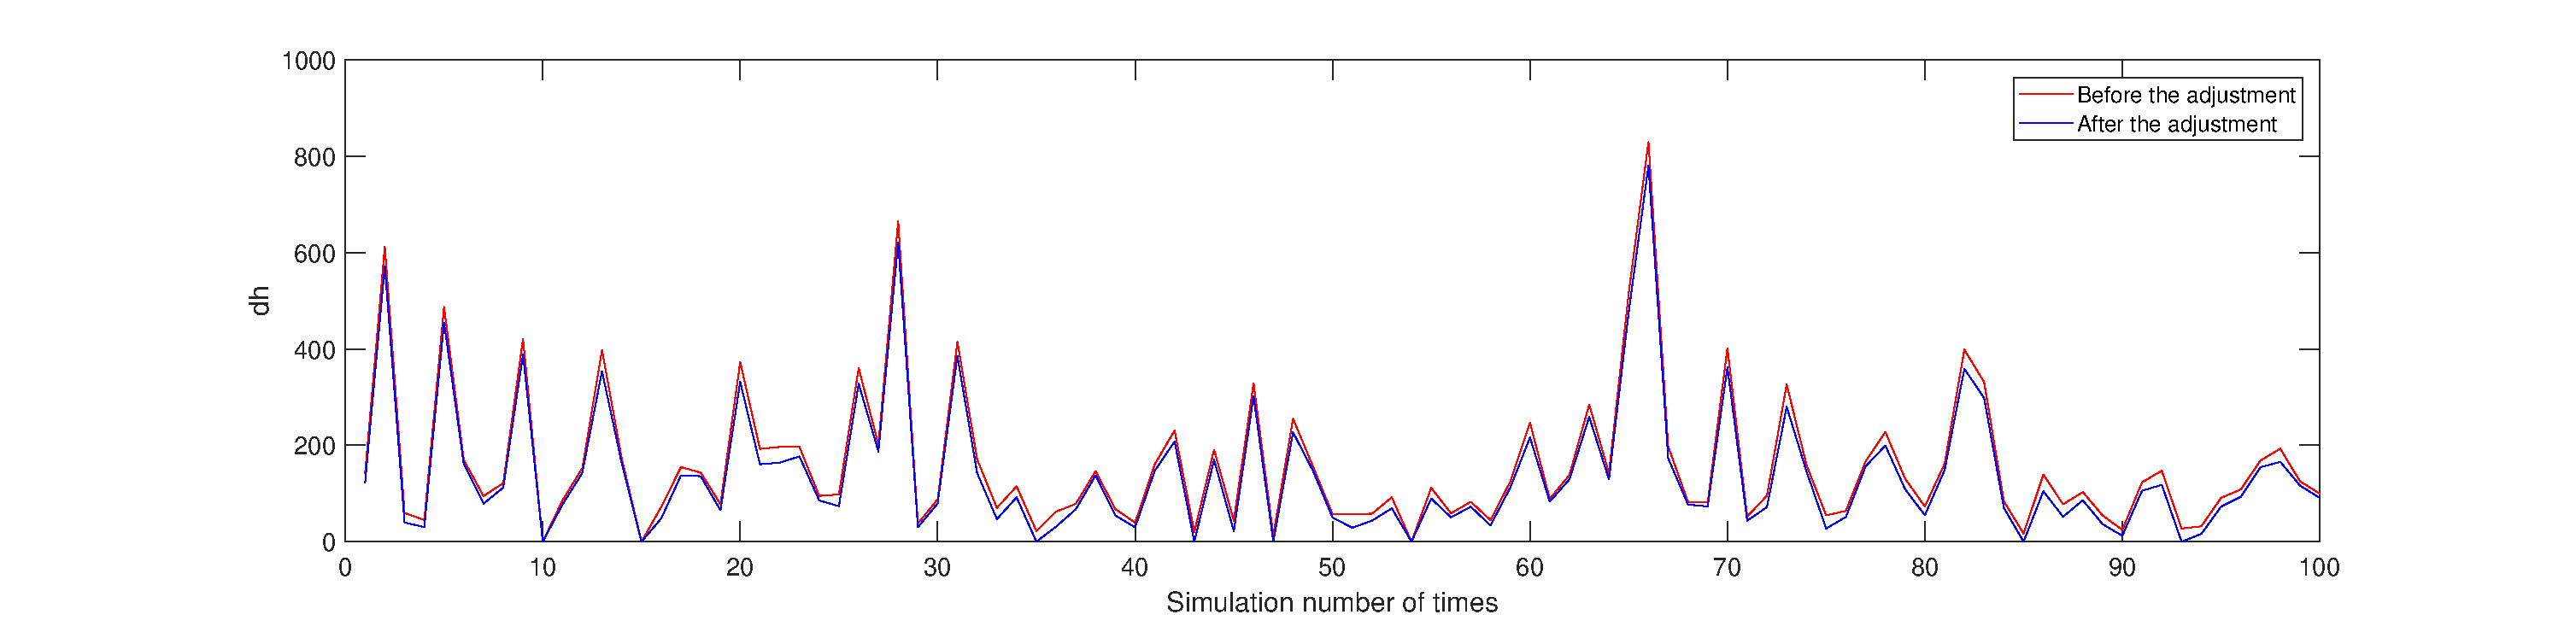
\includegraphics[width=14cm]{S1_2_1.eps}
					\caption{Enthalpy difference of each group before and after adjustment} \label{fig:2}
				\end{figure}
			
				In figure \ref{fig:2.1}, We calculated the reduced enthalpy difference of each group of data after adjustment. We can see that our algorithm significantly reduced the enthalpy difference, that is, significantly reduced the power consumption of the thermostat in the maintenance phase.
				
				\begin{figure}[h]
					\small
					\centering
					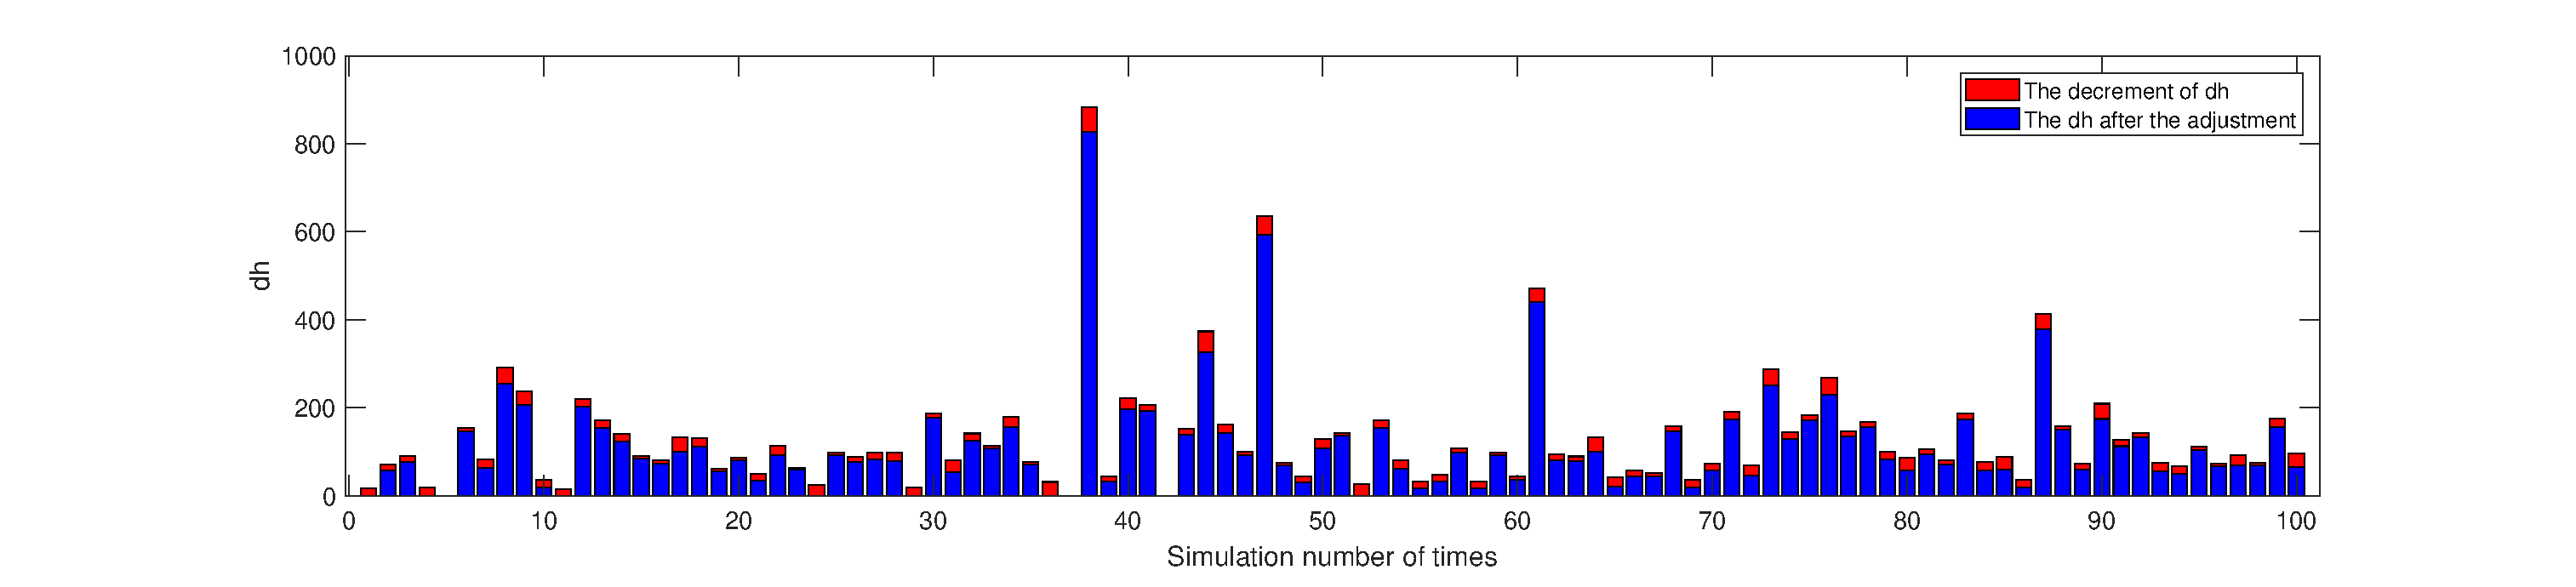
\includegraphics[width=14cm]{S1_2_2.eps}
					\caption{Reduced enthalpy difference of each group} \label{fig:2.1}
				\end{figure}
			
				In order to calculate the ratio of our algorithm to reduce the power consumption of thermostat, we simulated 1000 sets of data.
				
				The results show that the average enthalpy difference before and after adjustment is 153.9255, 134.1903 and 19.7252, which reduces the power consumption of the thermostat at the maintenance temperature stage by 12.82\%.
			
			
		\subsection{Task 2: Simulations under Muti-Dwellers}
			\subsubsection{Input Data}	
				\begin{itemize}
					\item The hypothesis of group comfort and effective temperature and humidity has been introduced in detail in this model.
					
					\item Random generation of environmental temperature data of 5-35 degrees Celsius and environmental relative humidity data of 30-80\% in non-extreme environments.
					
					\item We suppose to ignore the slight changes that may occur in the atmosphere, and calculate the values.
				\end{itemize}	
				
			\subsubsection{Simulation}	
				In figure \ref{fig:3}, the red range of the figure below is based on the constraints of temperature and humidity drawn by the group comfortable effective temperature line. The'*'point is the simulated environmental temperature and humidity, and the'+' point at the other end of the line is the optimal adjusted temperature and humidity result calculated by the system.
				
				\begin{figure}[h]
					\small
					\centering
					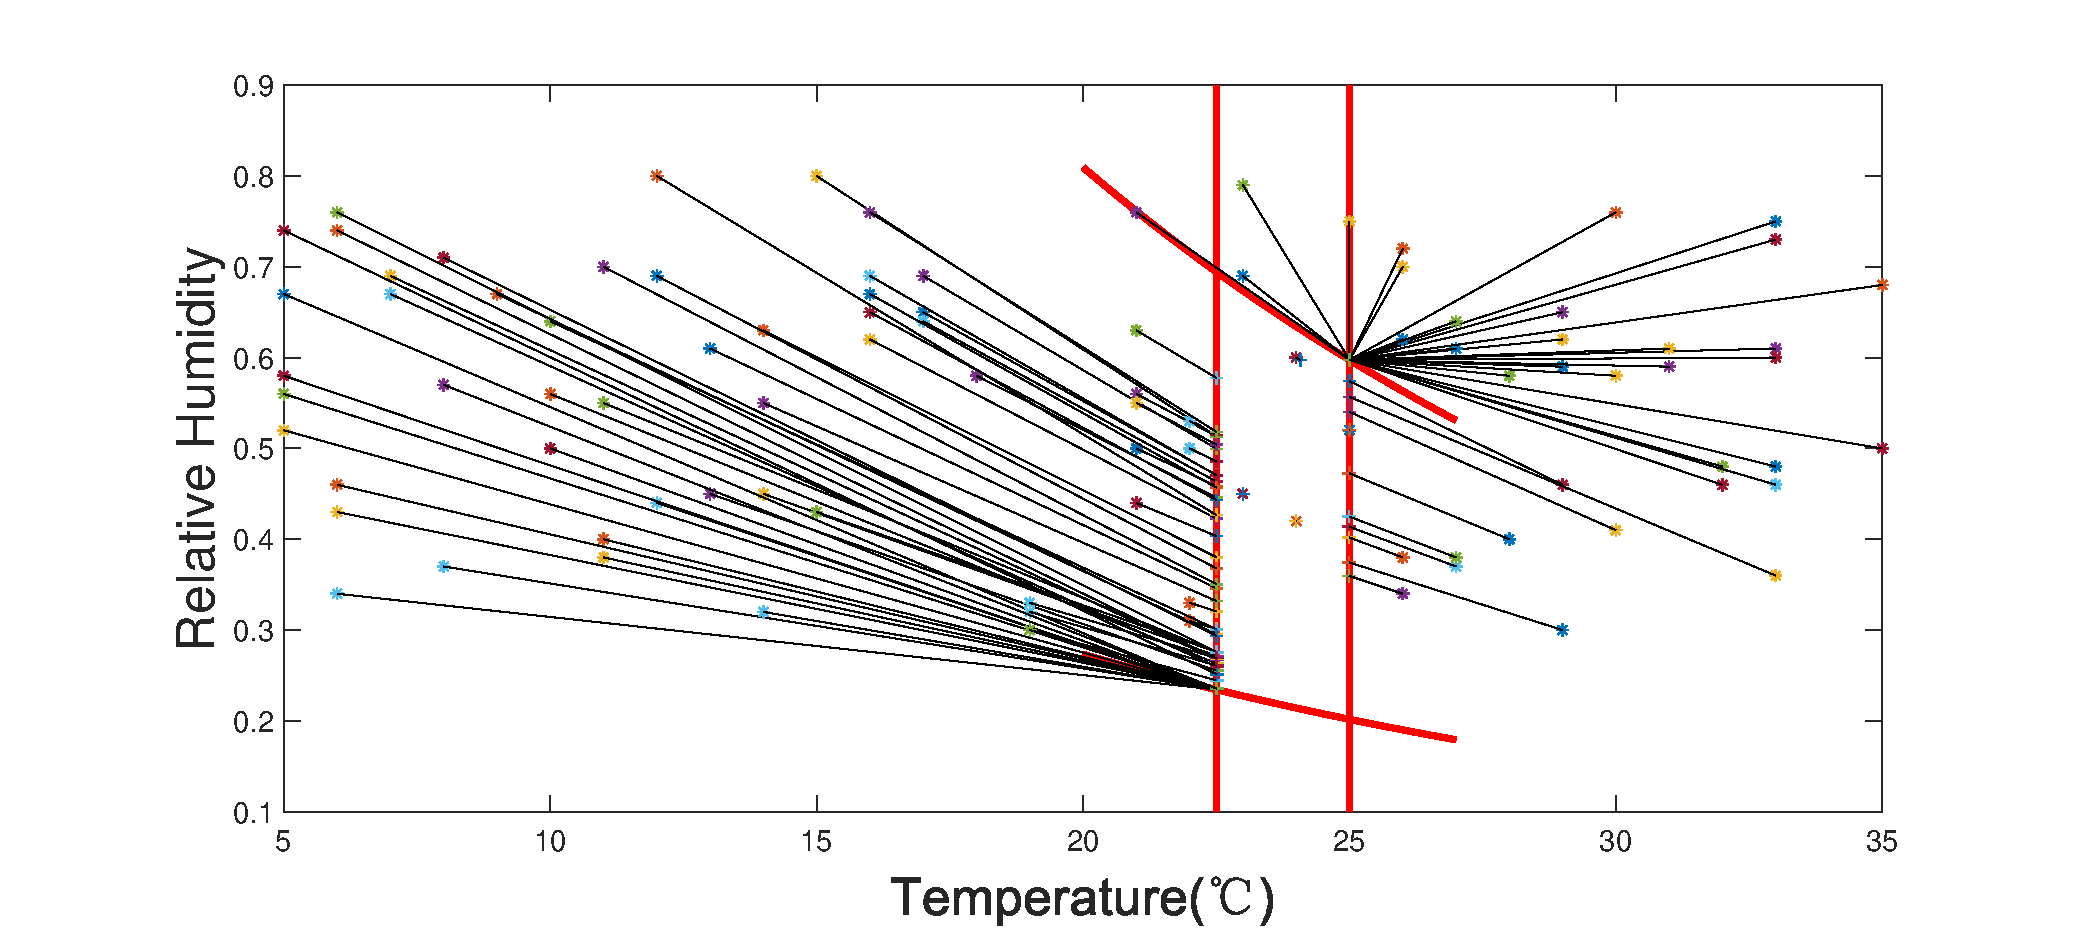
\includegraphics[width=14cm]{S2.eps}
					\caption{The minimum power consumption of the thermostat, and achieve the effect of group comfort} \label{fig:3}
				\end{figure}
				
				"+" is within the confining range, which proves that the adjusted temperature and humidity have reached group comfort. The adjustment strategy can minimize the enthalpy difference required to adjust temperature and humidity, that is, to meet the minimum power consumption of the thermostat, and achieve the effect of group comfort. 
	
	\section{Comparison with systems currently in use}
		\subsection{Review of existing systems}
		
			When it comes to smart thermostats, there’s a handful to choose from, but the big three that stand out are the Nest, Ecobee4, and Honeywell Lyric Round.
			\footnote{The Ontario Government of Canada has an energy conservation program that provides free smart networked thermostats for qualified users. For more imformation, please visit the website: https://www.greenon.ca/}
			Here we will elaborate on their advantages and characteristics relative to the rest of the products.
			
			\textbf{What They All Have in Common:}
			
			\begin{itemize}
				\item When you are away from home, you can control thermostats with mobile phones.
				
				\item Provide a programmable interface to users, so that users can set the time to open or close, and set the temperature value.
				
				\item Geofencing and motion detection, so it knows when you’re home.This function makes people do not need to start manually after getting home.
				
				\item Some humanized designs, such as voice and dialogue, and weather forecasts.
			\end{itemize}
			
			\textbf{Some unique designs made them popular:}
			
			\begin{itemize}
				\item \textbf{Nest}
				
				Nest provides a learning mechanism to learn your setting habits from your historical data and to simulate your habits for automatic setting. 
				These include automatically setting the start/end time, and the  temperature settings.
				
				\item \textbf{Ecobee4}
				
				However, the Ecobee4 has a wireless remote sensor that you can place anywhere. In this case, it works best placed upstairs where the temperature differs. From there, you can tell your Ecobee4 to use the sensor upstairs in order to gauge whether the A/C or heat should be running or not.
				
				Of course, you can simply just crank up any other thermostat to compensate for the warmer upstairs region, but the Ecobee4’s remote sensor makes it precise so that you’re not wasting more energy than necessary.
				
			\end{itemize}
		
		
		\subsection{Comparison}
			\subsubsection{The Heating Process}
				By understanding the climate control system on the market, they all learn the master's daily behavior first and then achieve "intelligence", their learning methods are mainly two kinds of "speed" and "energy-saving".
				
				But both of them have shortcomings, "speed" systems can basically meet the comfort needs of users, but due to changes in weather and other factors, the lack of timely reflection will lead to waste of energy.
				
				"Energy-saving" type is to learn the master's setting time, find out the most suitable and energy-saving situation in many cases corresponding to the opening time, but many times can not meet the master's comfort requirements.
				
				\textbf{Our system has made a thorough improvement on this issue. After learning the user's historical data, we synthesized real-time data, which saved the waste of resources caused by uncontrollable factors and made it comfortable as well.}
				
			\subsubsection{The Maintaining Process}
				The air-conditioning system on the market will generally remain in the current state after reaching the optimum conditions set by the owner. It will not consider how to control temperature and humidity to reduce energy consumption when reaching the optimum conditions.
				
				After reaching the optimum temperature set by the host, our system will monitor the current environmental variables in real time, adjust the temperature and humidity appropriately according to the changes of the environment, and minimize the energy consumption without obvious changes in temperature, humidity or comfort.
				
				But the system on the market takes into account the uneven temperature in the room. It allows you to adjust the temperature according to the installation location of the sensor. This is not considered by our system, but also can be improved.
				
				\textbf{In summary, our system takes into account the dynamic adjustment of temperature and humidity combination in a constant temperature state to reduce energy consumption. This is a progress, but it fails to take into account the negative impact of uneven climate in the room.}
	
	\section{Muti-Thermostrat linkage work}
	
		\subsection{Modeling Muti-Thermostrat linkage work}
			In this model, we mainly discuss the joint operation of multiple rooms (multiple thermostats).	That is to say, we need a general control algorithm to dynamically plan and guide the work of each thermostat. The working principle is as follows:
			
			\begin{figure}[h]
				\small
				\centering
				\includegraphics[width=12cm]{MM1.pdf}
				\caption{Relationship among the Models} \label{fig:process2}
			\end{figure}
			
			Because our smart climate control system used to obtain environmental parameters through outdoor and indoor sensors, but in the case of multiple thermostats, because not only the outdoor environment has an impact on the house, other rooms will also affect the house accordingly.
			
			Therefore, besides installing sensors outdoors, we also need to install sensors in adjacent rooms or allow multiple sensors to interconnect, and then get the temperature, humidity and other data of each room.
			
			According to each person's schedule, expected temperature, as well as the corresponding room (separate space), the location of public space (adjacent relationship) We can get the expected temperature for each house at a specific time. On this basis, we can analyze the temperature transfer in any room at any time. 
			
			Considering the interaction of multiple rooms, we can make the thermostat work in coordination through dynamic analysis at each time. Low power control air conditioning works to maintain temperature. For each room, there are three senarios:
			
			\begin{itemize}
				\item \textbf{No one in the room.}\\
				At this time, the room is regarded as part of the environment. The temperature in the room is the same as that in the environment. The thermostat does not work and the air conditioning power is 0.
				
				\item \textbf{one in the room.}\\
				At this time, the room temperature should be considered as an environmental variable in the maintenance phase of model 1. The heat transfer power can be obtained and the air conditioning power needed to maintain the temperature can be obtained.
				
				\item \textbf{More than one in the room.}\\
				At this time, the optimal temperature regulation strategy can be obtained from model 2 when many people are in public space, and the temperature strategy can be used as the expected temperature of the room.
				
			\end{itemize}
		
			\begin{figure}[h]
				\small
				\centering
				\includegraphics[width=9cm]{MM2.pdf}
				\caption{Relationship for each room} \label{fig:process3}
			\end{figure}
		
			Solving this problem is a process of dynamic analysis.
			
			At some point, for a room, its optimal power conditioning strategy satisfies the following conditions:
			
			\begin{equation}
				P = Q_{heat\ transfer\ to\ the\ environment} + \sum_{i=1}^m Q_{adjacent\ rooms\ heat\ transfer}
			\end{equation}
			
			By synthesizing the expected temperature of each room at every moment, we can find the minimum power consumption required for the thermostats to work together to maintain the temperature.
			

		\subsection{Simulations under Muti-Thermostrat}
			\subsubsection{Input Data}
			
				
			
				\begin{itemize}
					\item The daily schedule of three people and the different temperature preferences at different time periods were simulated reasonably.
					
					\item Take the actual temperature and humidity change of 24h in Chengdu as the environmental temperature and humidity change.
					
				\end{itemize}
			
				\begin{figure}[h]
					\small
					\centering
					\includegraphics[width=14cm]{MS1.pdf}
					\caption{System Structure for Four Romm} 
					\label{fig:room}
				\end{figure}
			
				\begin{itemize}	
				
					\item Assuming that there are four houses (room chart) with the following location relationship, only hypothetical walls exist among the houses, but no windows, doors and other thermal conductive structures are considered. Reasonable assumptions are made on the length, width and height of the building and the heat transfer coefficient of the wall surface.
					
					\item A,B and C three people are separately living in room 1,2 and 3, while room 4 is public space.
					
				\end{itemize}
			
				
			
			\subsubsection{Simulation}
				Firstly, in fugure \ref{fig:M4_P}, we combined three people's schedules and different temperature preferences in different time periods to get the following data.
				
				\begin{figure}[htb]
					\small
					\centering
					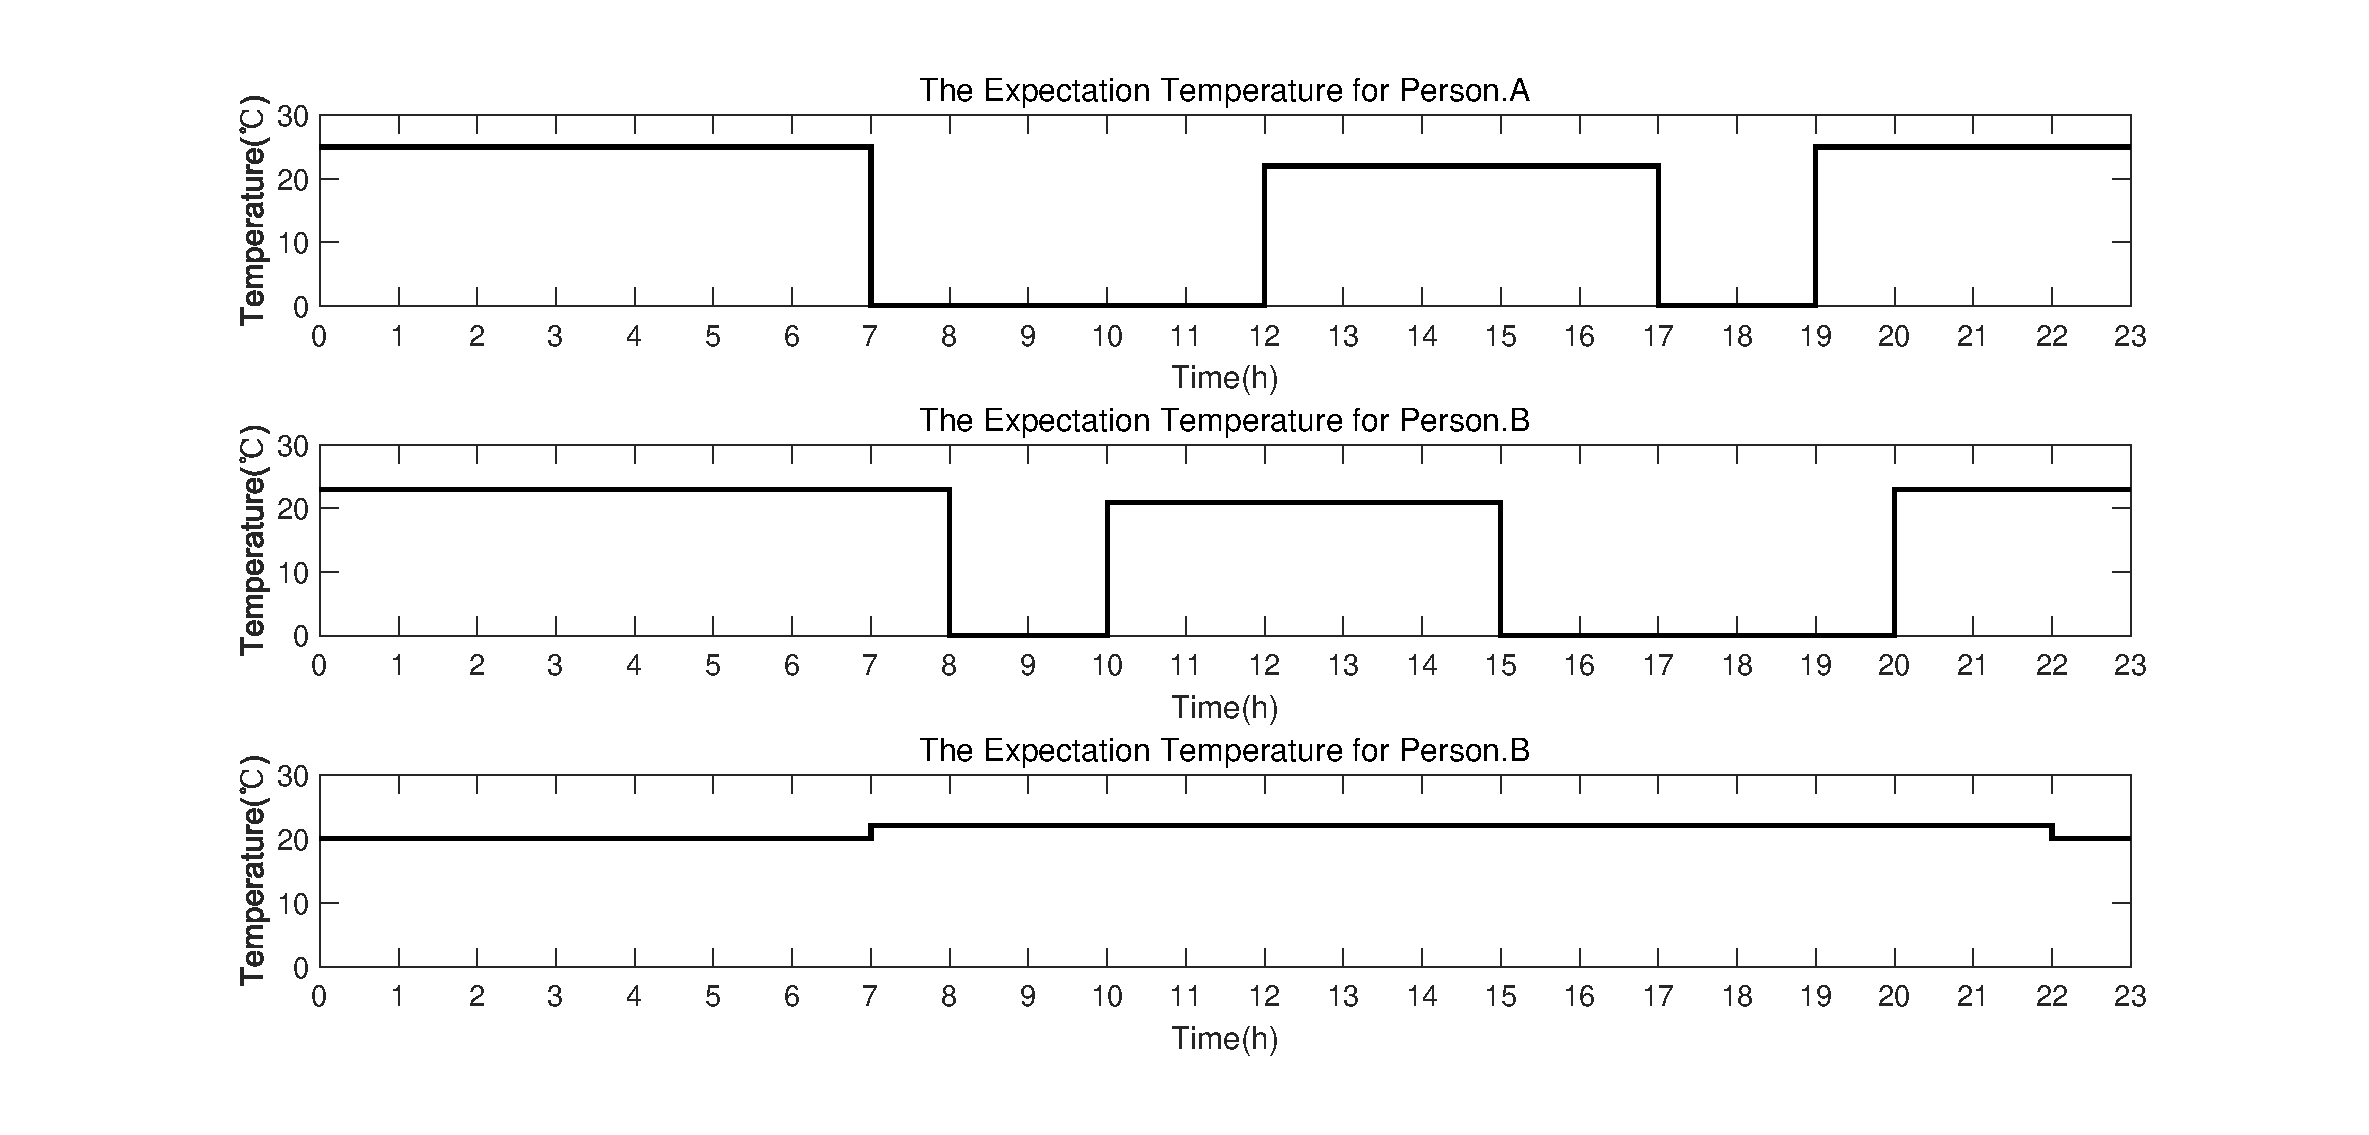
\includegraphics[width=14cm]{MS2.eps}
					\caption{Three people's schedules and preferences in different time periods} \label{fig:M4_P}
				\end{figure}
			
				The temperature of four rooms on the left varies with time, while the power required to change the room on the right varies with time. 
				
				\begin{figure}[h]
					\small
					\centering
					\includegraphics[width=14cm]{MS3_1.eps}
					\caption{Room-1} 
					\label{fig:M4_R1}
				\end{figure}
				\begin{figure}[H]
					\small
					\centering
					\includegraphics[width=14cm]{MS3_2.eps}
					\caption{Room-2} 
					\label{fig:M4_R2}
				\end{figure}
				\begin{figure}[htbp]
					\small
					\centering
					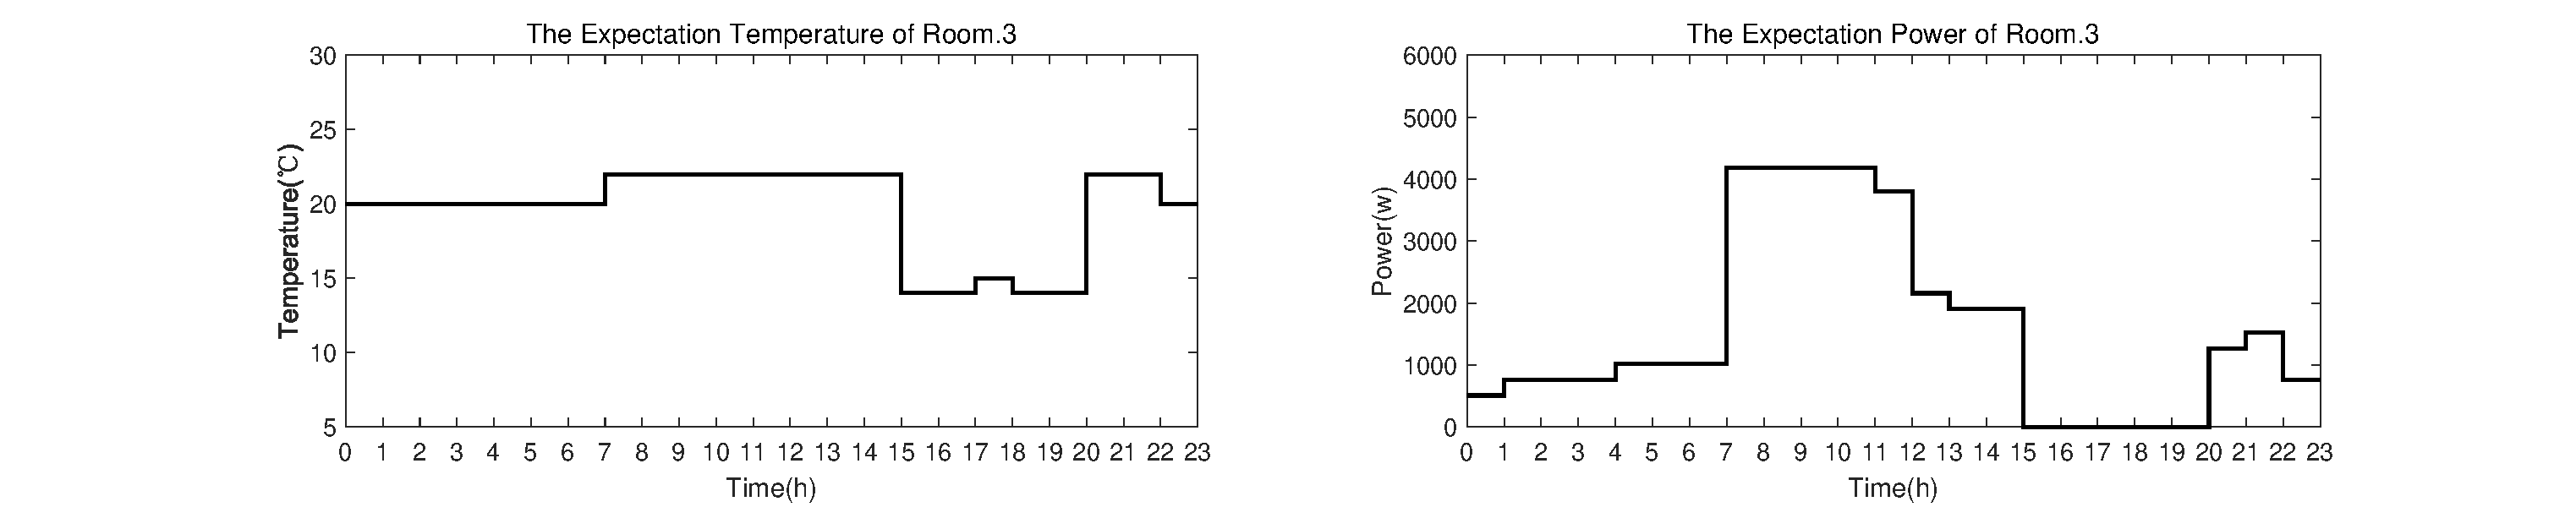
\includegraphics[width=14cm]{MS3_3.eps}
					\caption{Room-3} 
					\label{fig:M4_R3}
				\end{figure}
				\begin{figure}[H]
					\small
					\centering
					\includegraphics[width=14cm]{MS3_4.eps}
					\caption{Room-4} 
					\label{fig:M4_R4}
				\end{figure}
			
				
				In the same room at the same temperature, the power is also changing, which is the result of the coordinating work of the thermostat.
				
				
	
	\section{Sensitivity Analysis}
	
		We believe that in our system, one-to-one is the most basic part and the key of the whole model, so we make sensitivity analysis of one-to-one maintenance temperature part.
		
		We first changed the temperature range allowed to adjust, from the initial 1 degrees Celsius to 1.5, 2,2.5,3.
		
		The following figure shows the result in figure \ref{fig:s1}. We can see that with the increase of the allowable range of temperature adjustment, the difference of DH increases gradually. This is in line with our model, but with the further increase of the adjustable range of temperature, the difference of DH does not increase any more, because the effect of temperature adjustment on DH is small, which is also in line with our model.
		
		\begin{figure}[htbp]
			\small
			\centering
			\includegraphics[width=12cm]{Si1.png}
			%\caption{} 
			\label{fig:s1}
		\end{figure}
		
		We will then change the scope of PMV allowed to change from the original 0.5 to 0.7,1,1.2,1.5.
		
		The following figure \ref{fig:s2} shows the result. We can see that with the increase of the allowable range of PMV adjustment, the difference after DH adjustment basically does not change. This is because PMV is determined by both humidity and temperature. Humidity has little effect on PMV and temperature has a great influence on PMV. For dh, humidity has a great influence on DH and temperature has little effect on dh, so PMV can be adjusted. The change of scope does not allow DH to adjust the difference obviously, which is also consistent with our model. 
		
		\begin{figure}[htbp]
			\small
			\centering
			\includegraphics[width=12cm]{Si2.png}
			%\caption{} 
			\label{fig:s2}
		\end{figure}
		
		
	

	
	\section{Strengths and Weaknesses}
	
		\subsection{Strengths}
		
			\begin{itemize}
				
				\item \textbf{Scientific Modeling}\\
				We take full account of human shortcomings and the negative impact of habits, and innovatively integrate human preferences with theoretical and real-time data.
				
				\item \textbf{Coverage}\\
				Our model and measures are capable of simulating various scenarios associated with different external environment variables,geographical position.
				
				\item \textbf{Flexibility}\\
				Our model can be easily incorporated with other assumptions. For example, if we assume that an individual has another requires , our model can be modified to cover this assumption simply by adding constraints on the most suitable area.
				
				\item \textbf{Appealing Simulation Results}\\
				Simulation results of our model are very appealing.
				Not only do them effectively reflect the improvement of our system, but they present insightful adaptation for the changes on  household in-door situation. 
				In the case of Task 3, we discovered that applying co-operative thermostatic control system leads to effectively lower power consumption.
		
			\end{itemize}
		
		\subsection{Weaknesses}
		
			\begin{itemize}
				
				\item \textbf{Simulation Volatility}\\
				Although our model has thoughtful consideration, results generated by different simulations suffer high volatility.
				One possible remedy is to expand the number of samples, which reduces outcome variance at the cost of computational resources.
				
				\item \textbf{Unrealistic assumptions}\\
				In order to make the model easy to simulate, when we consider the temperature, especially the ambient temperature, we all think that it is a fixed value for a period of time, which is impossible in reality. At the same time, it is unrealistic to assume that the room temperature immediately restores to the same temperature as the ambient temperature after people leave.
				
				\item \textbf{Incomplete assumptions}\\
				There are many factors that we do not take into account, such as in the heating model, we neglect the heat storage and the objective heat dissipation of windows, roofs and so on.
				
			\end{itemize}
		
	\section{Conclusions}
	
		Up to now, we have accomplished all our tasks. And here we give the overall results of all our models.
		
		Above all, we propose two algorithms to solve the situation of a person in a room and multiple dwellers in a room. The algorithm not only considers the household's preference for temperature and other factors, but also uses theoretical knowledge and real-time data for multi-objective optimization. Finally, the impact of the user's special preferences such as air pollution level on the model is considered. 
		
		Then we propose a model that enables multiple thermostats to work together, which gives us the opportunity to consider the interaction between the thermostats in oder to further reduce energy consumption while ensuring comfort as well.
		
		As we consider various different conditions and analyze the simulation results we can conclude that:
		
		\begin{itemize}
			\item The system under this model is fairly stable with different variables.
			
			\item The model has better improvement compared with the strategies currently used.
			
			\item The model also needs better assumptions and more robust simulation data.
		\end{itemize}

	\nocite{*}
	\bibliography{reference,cnki}
	
	\newpage
	\section{News Release}
	
		
		
		
		\begin{center}
			\Large\textbf{A Novel Thermostat: Born to Know You Better}
			
			\emph{To all interested users}
		\end{center}
		
		Have you ever been struggling between saving electricity and early opening air conditioner before you got home? 
		
		Have you ever had no idea how to regulate air conditioners when multiple people live together?
		
		We found out a technical design to solve these problems once for all! Let’s catch a glimpse of this thermostat now! 
		
		At first, we find a novel approach to better control the indoor climate (including factors such as temperature and humidity) in order to achieve the most comfortable condition for you, and better power saving at the same time. When the thermostat knows your schedule, it can take the outdoor climate of the day into account and adjust the time to turn on the air conditioner no matter how different the previous schedule is. It is because the thermostat can be arranged according to the real-time situation around it, so it can also save more power.
		
		As for the situation when many people are in the same room, The thermostat intelligently abandons personal preferences (taking into account the fairness and comfort for more people) to regulate the temperature and humidity. In addition, within the range of combinations of parameter that make the group feel most comfortable, it can intelligently select the certain parameter setting with the least energy consumption.
		
		We also considered the combined working status of multiple thermostats, if you install more than one thermostat for rooms in your home. We can automatically consider the heat transfer in rooms and use less energy to get your environment to your demands.
		
		As we all know, a more comfortable indoor climate means more energy consumption, we not just guarantee a comfortable indoor climate, but also a promise of energy-saving.
		
		Unlike existing smart thermostats, our novel thermostat not only “learn” from you, it also “learn” from theoretical and real-time environmental data, which allows it to better manage your living environment after understanding your preferences. Because it senses the environment more accurately, it could know you better than yourself.
		
		All we have done is to give users a better combination of theoretical optimality and personal preference.
		
			
		
	
	


\end{document}
